\documentclass[1p]{elsarticle_modified}
%\bibliographystyle{elsarticle-num}

%\usepackage[colorlinks]{hyperref}
%\usepackage{abbrmath_seonhwa} %\Abb, \Ascr, \Acal ,\Abf, \Afrak
\usepackage{amsfonts}
\usepackage{amssymb}
\usepackage{amsmath}
\usepackage{amsthm}
\usepackage{scalefnt}
\usepackage{amsbsy}
\usepackage{kotex}
\usepackage{caption}
\usepackage{subfig}
\usepackage{color}
\usepackage{graphicx}
\usepackage{xcolor} %% white, black, red, green, blue, cyan, magenta, yellow
\usepackage{float}
\usepackage{setspace}
\usepackage{hyperref}

\usepackage{tikz}
\usetikzlibrary{arrows}

\usepackage{multirow}
\usepackage{array} % fixed length table
\usepackage{hhline}

%%%%%%%%%%%%%%%%%%%%%
\makeatletter
\renewcommand*\env@matrix[1][\arraystretch]{%
	\edef\arraystretch{#1}%
	\hskip -\arraycolsep
	\let\@ifnextchar\new@ifnextchar
	\array{*\c@MaxMatrixCols c}}
\makeatother %https://tex.stackexchange.com/questions/14071/how-can-i-increase-the-line-spacing-in-a-matrix
%%%%%%%%%%%%%%%

\usepackage[normalem]{ulem}

\newcommand{\msout}[1]{\ifmmode\text{\sout{\ensuremath{#1}}}\else\sout{#1}\fi}
%SOURCE: \msout is \stkout macro in https://tex.stackexchange.com/questions/20609/strikeout-in-math-mode

\newcommand{\cancel}[1]{
	\ifmmode
	{\color{red}\msout{#1}}
	\else
	{\color{red}\sout{#1}}
	\fi
}

\newcommand{\add}[1]{
	{\color{blue}\uwave{#1}}
}

\newcommand{\replace}[2]{
	\ifmmode
	{\color{red}\msout{#1}}{\color{blue}\uwave{#2}}
	\else
	{\color{red}\sout{#1}}{\color{blue}\uwave{#2}}
	\fi
}

\newcommand{\Sol}{\mathcal{S}} %segment
\newcommand{\D}{D} %diagram
\newcommand{\A}{\mathcal{A}} %arc


%%%%%%%%%%%%%%%%%%%%%%%%%%%%%5 test

\def\sl{\operatorname{\textup{SL}}(2,\Cbb)}
\def\psl{\operatorname{\textup{PSL}}(2,\Cbb)}
\def\quan{\mkern 1mu \triangleright \mkern 1mu}

\theoremstyle{definition}
\newtheorem{thm}{Theorem}[section]
\newtheorem{prop}[thm]{Proposition}
\newtheorem{lem}[thm]{Lemma}
\newtheorem{ques}[thm]{Question}
\newtheorem{cor}[thm]{Corollary}
\newtheorem{defn}[thm]{Definition}
\newtheorem{exam}[thm]{Example}
\newtheorem{rmk}[thm]{Remark}
\newtheorem{alg}[thm]{Algorithm}

\newcommand{\I}{\sqrt{-1}}
\begin{document}

%\begin{frontmatter}
%
%\title{Boundary parabolic representations of knots up to 8 crossings}
%
%%% Group authors per affiliation:
%\author{Yunhi Cho} 
%\address{Department of Mathematics, University of Seoul, Seoul, Korea}
%\ead{yhcho@uos.ac.kr}
%
%
%\author{Seonhwa Kim} %\fnref{s_kim}}
%\address{Center for Geometry and Physics, Institute for Basic Science, Pohang, 37673, Korea}
%\ead{ryeona17@ibs.re.kr}
%
%\author{Hyuk Kim}
%\address{Department of Mathematical Sciences, Seoul National University, Seoul 08826, Korea}
%\ead{hyukkim@snu.ac.kr}
%
%\author{Seokbeom Yoon}
%\address{Department of Mathematical Sciences, Seoul National University, Seoul, 08826,  Korea}
%\ead{sbyoon15@snu.ac.kr}
%
%\begin{abstract}
%We find all boundary parabolic representation of knots up to 8 crossings.
%
%\end{abstract}
%\begin{keyword}
%    \MSC[2010] 57M25 
%\end{keyword}
%
%\end{frontmatter}

%\linenumbers
%\tableofcontents
%
\newcommand\colored[1]{\textcolor{white}{\rule[-0.35ex]{0.8em}{1.4ex}}\kern-0.8em\color{red} #1}%
%\newcommand\colored[1]{\textcolor{white}{ #1}\kern-2.17ex	\textcolor{white}{ #1}\kern-1.81ex	\textcolor{white}{ #1}\kern-2.15ex\color{red}#1	}

{\Large $\underline{12n_{0860}~(K12n_{0860})}$}

\setlength{\tabcolsep}{10pt}
\renewcommand{\arraystretch}{1.6}
\vspace{1cm}\begin{tabular}{m{100pt}>{\centering\arraybackslash}m{274pt}}
\multirow{5}{120pt}{
	\centering
	\includegraphics[width=112pt]{../../../GIT/diagram.site/Diagrams/png/2949_12n_0860.png}\\
\ \ \ A knot diagram\footnotemark}&
\allowdisplaybreaks
\textbf{Linearized knot diagam} \\
\cline{2-2}
 &
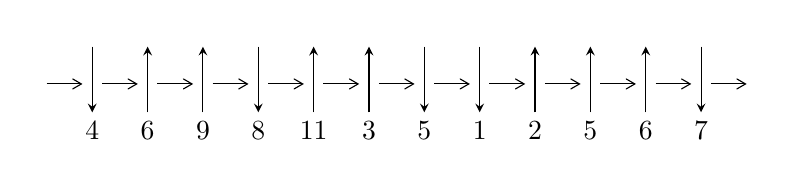
\begin{tikzpicture}[x=20pt, y=17pt]
	% nodes
	\node (C0) at (0, 0) {};
	\node (C1) at (1, 0) {};
	\node (C1U) at (1, +1) {};
	\node (C1D) at (1, -1) {4};

	\node (C2) at (2, 0) {};
	\node (C2U) at (2, +1) {};
	\node (C2D) at (2, -1) {6};

	\node (C3) at (3, 0) {};
	\node (C3U) at (3, +1) {};
	\node (C3D) at (3, -1) {9};

	\node (C4) at (4, 0) {};
	\node (C4U) at (4, +1) {};
	\node (C4D) at (4, -1) {8};

	\node (C5) at (5, 0) {};
	\node (C5U) at (5, +1) {};
	\node (C5D) at (5, -1) {11};

	\node (C6) at (6, 0) {};
	\node (C6U) at (6, +1) {};
	\node (C6D) at (6, -1) {3};

	\node (C7) at (7, 0) {};
	\node (C7U) at (7, +1) {};
	\node (C7D) at (7, -1) {5};

	\node (C8) at (8, 0) {};
	\node (C8U) at (8, +1) {};
	\node (C8D) at (8, -1) {1};

	\node (C9) at (9, 0) {};
	\node (C9U) at (9, +1) {};
	\node (C9D) at (9, -1) {2};

	\node (C10) at (10, 0) {};
	\node (C10U) at (10, +1) {};
	\node (C10D) at (10, -1) {5};

	\node (C11) at (11, 0) {};
	\node (C11U) at (11, +1) {};
	\node (C11D) at (11, -1) {6};

	\node (C12) at (12, 0) {};
	\node (C12U) at (12, +1) {};
	\node (C12D) at (12, -1) {7};
	\node (C13) at (13, 0) {};

	% arrows
	\draw[->,>={angle 60}]
	(C0) edge (C1) (C1) edge (C2) (C2) edge (C3) (C3) edge (C4) (C4) edge (C5) (C5) edge (C6) (C6) edge (C7) (C7) edge (C8) (C8) edge (C9) (C9) edge (C10) (C10) edge (C11) (C11) edge (C12) (C12) edge (C13) ;	\draw[->,>=stealth]
	(C1U) edge (C1D) (C2D) edge (C2U) (C3D) edge (C3U) (C4U) edge (C4D) (C5D) edge (C5U) (C6D) edge (C6U) (C7U) edge (C7D) (C8U) edge (C8D) (C9D) edge (C9U) (C10D) edge (C10U) (C11D) edge (C11U) (C12U) edge (C12D) ;
	\end{tikzpicture} \\
\hhline{~~} \\& 
\textbf{Solving Sequence} \\ \cline{2-2} 
 &
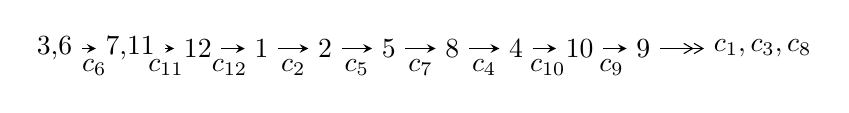
\begin{tikzpicture}[x=23pt, y=7pt]
	% node
	\node (A0) at (-1/8, 0) {3,6};
	\node (A1) at (17/16, 0) {7,11};
	\node (A2) at (17/8, 0) {12};
	\node (A3) at (25/8, 0) {1};
	\node (A4) at (33/8, 0) {2};
	\node (A5) at (41/8, 0) {5};
	\node (A6) at (49/8, 0) {8};
	\node (A7) at (57/8, 0) {4};
	\node (A8) at (65/8, 0) {10};
	\node (A9) at (73/8, 0) {9};
	\node (C1) at (1/2, -1) {$c_{6}$};
	\node (C2) at (13/8, -1) {$c_{11}$};
	\node (C3) at (21/8, -1) {$c_{12}$};
	\node (C4) at (29/8, -1) {$c_{2}$};
	\node (C5) at (37/8, -1) {$c_{5}$};
	\node (C6) at (45/8, -1) {$c_{7}$};
	\node (C7) at (53/8, -1) {$c_{4}$};
	\node (C8) at (61/8, -1) {$c_{10}$};
	\node (C9) at (69/8, -1) {$c_{9}$};
	\node (A10) at (11, 0) {$c_{1},c_{3},c_{8}$};

	% edge
	\draw[->,>=stealth]	
	(A0) edge (A1) (A1) edge (A2) (A2) edge (A3) (A3) edge (A4) (A4) edge (A5) (A5) edge (A6) (A6) edge (A7) (A7) edge (A8) (A8) edge (A9) ;
	\draw[->>,>={angle 60}]	
	(A9) edge (A10);
\end{tikzpicture} \\ 

\end{tabular} \\

\footnotetext{
The image of knot diagram is generated by the software ``\textbf{Draw programme}" developed by Andrew Bartholomew(\url{http://www.layer8.co.uk/maths/draw/index.htm\#Running-draw}), where we modified some parts for our purpose(\url{https://github.com/CATsTAILs/LinksPainter}).
}\phantom \\ \newline 
\centering \textbf{Ideals for irreducible components\footnotemark of $X_{\text{par}}$} 
 
\begin{align*}
I^u_{1}&=\langle 
b+u,\;-6573198 u^{24}-7407745 u^{23}+\cdots+830359 a-20171003,\;u^{25}-6 u^{23}+\cdots+10 u^2-1\rangle \\
I^u_{2}&=\langle 
4.04286\times10^{177} u^{71}-1.22456\times10^{178} u^{70}+\cdots+1.03797\times10^{179} b+1.12104\times10^{180},\\
\phantom{I^u_{2}}&\phantom{= \langle  }2.07451\times10^{180} u^{71}-5.60040\times10^{180} u^{70}+\cdots+6.92329\times10^{181} a+4.53244\times10^{182},\\
\phantom{I^u_{2}}&\phantom{= \langle  }u^{72}-2 u^{71}+\cdots+3115 u+667\rangle \\
I^u_{3}&=\langle 
b+u,\;3 u^{13}- u^{12}-10 u^{11}+7 u^{10}+16 u^9-21 u^8-13 u^7+31 u^6-7 u^5-19 u^4+17 u^3-2 u^2+a-3 u+3,\\
\phantom{I^u_{3}}&\phantom{= \langle  }u^{14}-4 u^{12}+u^{11}+8 u^{10}-5 u^9-10 u^8+10 u^7+5 u^6-10 u^5+2 u^4+4 u^3-2 u^2+1\rangle \\
I^u_{4}&=\langle 
u^{11}- u^{10}-4 u^9+5 u^8+5 u^7-9 u^6-3 u^5+9 u^4+5 u^3-5 u^2+b-4 u+1,\\
\phantom{I^u_{4}}&\phantom{= \langle  }-8 u^{11}+3 u^{10}+34 u^9-20 u^8-51 u^7+43 u^6+45 u^5-44 u^4-61 u^3+a+28 u+8,\\
\phantom{I^u_{4}}&\phantom{= \langle  }u^{12}- u^{11}-4 u^{10}+5 u^9+5 u^8-9 u^7-3 u^6+9 u^5+5 u^4-5 u^3-4 u^2+u+1\rangle \\
\\
\end{align*}
\raggedright * 4 irreducible components of $\dim_{\mathbb{C}}=0$, with total 123 representations.\\
\footnotetext{All coefficients of polynomials are rational numbers. But the coefficients are sometimes approximated in decimal forms when there is not enough margin.}
\newpage
\renewcommand{\arraystretch}{1}
\centering \section*{I. $I^u_{1}= \langle b+u,\;-6.57\times10^{6} u^{24}-7.41\times10^{6} u^{23}+\cdots+8.30\times10^{5} a-2.02\times10^{7},\;u^{25}-6 u^{23}+\cdots+10 u^2-1 \rangle$}
\flushleft \textbf{(i) Arc colorings}\\
\begin{tabular}{m{7pt} m{180pt} m{7pt} m{180pt} }
\flushright $a_{3}=$&$\begin{pmatrix}0\\u\end{pmatrix}$ \\
\flushright $a_{6}=$&$\begin{pmatrix}1\\0\end{pmatrix}$ \\
\flushright $a_{7}=$&$\begin{pmatrix}1\\- u^2\end{pmatrix}$ \\
\flushright $a_{11}=$&$\begin{pmatrix}7.91609 u^{24}+8.92114 u^{23}+\cdots+10.3907 u+24.2919\\- u\end{pmatrix}$ \\
\flushright $a_{12}=$&$\begin{pmatrix}7.91609 u^{24}+8.92114 u^{23}+\cdots+9.39074 u+24.2919\\- u\end{pmatrix}$ \\
\flushright $a_{1}=$&$\begin{pmatrix}3.56601 u^{24}+5.57186 u^{23}+\cdots+2.47465 u+15.3708\\1.95267 u^{24}+1.21283 u^{23}+\cdots+3.35008 u+3.34927\end{pmatrix}$ \\
\flushright $a_{2}=$&$\begin{pmatrix}- u\\u\end{pmatrix}$ \\
\flushright $a_{5}=$&$\begin{pmatrix}-8.92114 u^{24}-4.35008 u^{23}+\cdots-24.2919 u-6.91609\\u^2\end{pmatrix}$ \\
\flushright $a_{8}=$&$\begin{pmatrix}-3.94984 u^{24}-1.36141 u^{23}+\cdots-15.3813 u-3.39671\\-1.21283 u^{24}-0.779766 u^{23}+\cdots-3.34927 u-1.95267\end{pmatrix}$ \\
\flushright $a_{4}=$&$\begin{pmatrix}-0.533909 u^{24}+2.27446 u^{23}+\cdots-10.2048 u+7.37157\\1.04484 u^{24}+0.684652 u^{23}+\cdots+1.56683 u+1.02792\end{pmatrix}$ \\
\flushright $a_{10}=$&$\begin{pmatrix}3.56601 u^{24}+5.57186 u^{23}+\cdots+3.47465 u+15.3708\\u^3- u\end{pmatrix}$ \\
\flushright $a_{9}=$&$\begin{pmatrix}1.16861 u^{24}+3.43542 u^{23}+\cdots-0.0913593 u+9.79891\\2.39741 u^{24}+2.13644 u^{23}+\cdots+2.56601 u+5.57186\end{pmatrix}$\\&\end{tabular}
\flushleft \textbf{(ii) Obstruction class $= -1$}\\~\\
\flushleft \textbf{(iii) Cusp Shapes $= -\frac{22412}{830359} u^{24}+\frac{3732748}{830359} u^{23}+\cdots-\frac{3546046}{830359} u+\frac{19755477}{830359}$}\\~\\
\newpage\renewcommand{\arraystretch}{1}
\flushleft \textbf{(iv) u-Polynomials at the component}\newline \\
\begin{tabular}{m{50pt}|m{274pt}}
Crossings & \hspace{64pt}u-Polynomials at each crossing \\
\hline $$\begin{aligned}c_{1},c_{8}\end{aligned}$$&$\begin{aligned}
&u^{25}- u^{24}+\cdots+2 u-1
\end{aligned}$\\
\hline $$\begin{aligned}c_{2},c_{5},c_{6}\\c_{10},c_{11}\end{aligned}$$&$\begin{aligned}
&u^{25}-6 u^{23}+\cdots+10 u^2-1
\end{aligned}$\\
\hline $$\begin{aligned}c_{3}\end{aligned}$$&$\begin{aligned}
&u^{25}-18 u^{24}+\cdots-144 u+32
\end{aligned}$\\
\hline $$\begin{aligned}c_{4},c_{7}\end{aligned}$$&$\begin{aligned}
&u^{25}-15 u^{24}+\cdots+864 u-64
\end{aligned}$\\
\hline $$\begin{aligned}c_{9}\end{aligned}$$&$\begin{aligned}
&u^{25}- u^{24}+\cdots+u-1
\end{aligned}$\\
\hline $$\begin{aligned}c_{12}\end{aligned}$$&$\begin{aligned}
&u^{25}+u^{24}+\cdots+48 u-19
\end{aligned}$\\
\hline
\end{tabular}\\~\\
\newpage\renewcommand{\arraystretch}{1}
\flushleft \textbf{(v) Riley Polynomials at the component}\newline \\
\begin{tabular}{m{50pt}|m{274pt}}
Crossings & \hspace{64pt}Riley Polynomials at each crossing \\
\hline $$\begin{aligned}c_{1},c_{8}\end{aligned}$$&$\begin{aligned}
&y^{25}+3 y^{24}+\cdots-18 y-1
\end{aligned}$\\
\hline $$\begin{aligned}c_{2},c_{5},c_{6}\\c_{10},c_{11}\end{aligned}$$&$\begin{aligned}
&y^{25}-12 y^{24}+\cdots+20 y-1
\end{aligned}$\\
\hline $$\begin{aligned}c_{3}\end{aligned}$$&$\begin{aligned}
&y^{25}+8 y^{24}+\cdots+28416 y-1024
\end{aligned}$\\
\hline $$\begin{aligned}c_{4},c_{7}\end{aligned}$$&$\begin{aligned}
&y^{25}+19 y^{24}+\cdots+9216 y-4096
\end{aligned}$\\
\hline $$\begin{aligned}c_{9}\end{aligned}$$&$\begin{aligned}
&y^{25}+7 y^{24}+\cdots-11 y-1
\end{aligned}$\\
\hline $$\begin{aligned}c_{12}\end{aligned}$$&$\begin{aligned}
&y^{25}+9 y^{24}+\cdots+860 y-361
\end{aligned}$\\
\hline
\end{tabular}\\~\\
\newpage\flushleft \textbf{(vi) Complex Volumes and Cusp Shapes}
$$\begin{array}{c|c|c}  
\text{Solutions to }I^u_{1}& \I (\text{vol} + \sqrt{-1}CS) & \text{Cusp shape}\\
 \hline 
\begin{aligned}
u &= \phantom{-}1.04100\phantom{ +0.000000I} \\
a &= \phantom{-}1.37005\phantom{ +0.000000I} \\
b &= -1.04100\phantom{ +0.000000I}\end{aligned}
 & \phantom{-}2.22466\phantom{ +0.000000I} & \phantom{-}3.28160\phantom{ +0.000000I} \\ \hline\begin{aligned}
u &= -0.988163 + 0.354424 I \\
a &= -0.606149 - 1.059700 I \\
b &= \phantom{-}0.988163 - 0.354424 I\end{aligned}
 & \phantom{-}7.43769 + 2.03575 I & \phantom{-}10.09013 + 0.83711 I \\ \hline\begin{aligned}
u &= -0.988163 - 0.354424 I \\
a &= -0.606149 + 1.059700 I \\
b &= \phantom{-}0.988163 + 0.354424 I\end{aligned}
 & \phantom{-}7.43769 - 2.03575 I & \phantom{-}10.09013 - 0.83711 I \\ \hline\begin{aligned}
u &= -1.064740 + 0.110709 I \\
a &= -2.02955 + 0.79466 I \\
b &= \phantom{-}1.064740 - 0.110709 I\end{aligned}
 & \phantom{-}5.86298 - 2.94895 I & \phantom{-}8.99062 + 3.88971 I \\ \hline\begin{aligned}
u &= -1.064740 - 0.110709 I \\
a &= -2.02955 - 0.79466 I \\
b &= \phantom{-}1.064740 + 0.110709 I\end{aligned}
 & \phantom{-}5.86298 + 2.94895 I & \phantom{-}8.99062 - 3.88971 I \\ \hline\begin{aligned}
u &= \phantom{-}0.773294 + 0.776856 I \\
a &= \phantom{-}0.399881 - 0.058553 I \\
b &= -0.773294 - 0.776856 I\end{aligned}
 & \phantom{-}2.95958 + 3.45034 I & \phantom{-}20.3542 + 1.7595 I \\ \hline\begin{aligned}
u &= \phantom{-}0.773294 - 0.776856 I \\
a &= \phantom{-}0.399881 + 0.058553 I \\
b &= -0.773294 + 0.776856 I\end{aligned}
 & \phantom{-}2.95958 - 3.45034 I & \phantom{-}20.3542 - 1.7595 I \\ \hline\begin{aligned}
u &= -0.701802 + 0.884948 I \\
a &= -1.189240 - 0.493880 I \\
b &= \phantom{-}0.701802 - 0.884948 I\end{aligned}
 & -1.69441 + 5.16318 I & \phantom{-}2.00598 - 2.40163 I \\ \hline\begin{aligned}
u &= -0.701802 - 0.884948 I \\
a &= -1.189240 + 0.493880 I \\
b &= \phantom{-}0.701802 + 0.884948 I\end{aligned}
 & -1.69441 - 5.16318 I & \phantom{-}2.00598 + 2.40163 I \\ \hline\begin{aligned}
u &= \phantom{-}0.926391 + 0.732700 I \\
a &= \phantom{-}1.176220 - 0.249303 I \\
b &= -0.926391 - 0.732700 I\end{aligned}
 & \phantom{-}0.74727 + 1.79853 I & \phantom{-}6.90577 + 1.84258 I\\
 \hline 
 \end{array}$$\newpage$$\begin{array}{c|c|c}  
\text{Solutions to }I^u_{1}& \I (\text{vol} + \sqrt{-1}CS) & \text{Cusp shape}\\
 \hline 
\begin{aligned}
u &= \phantom{-}0.926391 - 0.732700 I \\
a &= \phantom{-}1.176220 + 0.249303 I \\
b &= -0.926391 + 0.732700 I\end{aligned}
 & \phantom{-}0.74727 - 1.79853 I & \phantom{-}6.90577 - 1.84258 I \\ \hline\begin{aligned}
u &= \phantom{-}0.968203 + 0.709190 I \\
a &= \phantom{-}1.83876 - 0.47348 I \\
b &= -0.968203 - 0.709190 I\end{aligned}
 & -3.63929 + 1.05448 I & \phantom{-}1.231686 - 0.208690 I \\ \hline\begin{aligned}
u &= \phantom{-}0.968203 - 0.709190 I \\
a &= \phantom{-}1.83876 + 0.47348 I \\
b &= -0.968203 + 0.709190 I\end{aligned}
 & -3.63929 - 1.05448 I & \phantom{-}1.231686 + 0.208690 I \\ \hline\begin{aligned}
u &= \phantom{-}0.661030 + 0.060128 I \\
a &= \phantom{-}1.12111 - 4.60091 I \\
b &= -0.661030 - 0.060128 I\end{aligned}
 & \phantom{-}4.19613 - 4.91912 I & \phantom{-}7.66633 - 1.97464 I \\ \hline\begin{aligned}
u &= \phantom{-}0.661030 - 0.060128 I \\
a &= \phantom{-}1.12111 + 4.60091 I \\
b &= -0.661030 + 0.060128 I\end{aligned}
 & \phantom{-}4.19613 + 4.91912 I & \phantom{-}7.66633 + 1.97464 I \\ \hline\begin{aligned}
u &= -1.102000 + 0.839497 I \\
a &= -1.332340 - 0.405431 I \\
b &= \phantom{-}1.102000 - 0.839497 I\end{aligned}
 & -2.91779 - 11.36900 I & \phantom{-}2.13618 + 9.01386 I \\ \hline\begin{aligned}
u &= -1.102000 - 0.839497 I \\
a &= -1.332340 + 0.405431 I \\
b &= \phantom{-}1.102000 + 0.839497 I\end{aligned}
 & -2.91779 + 11.36900 I & \phantom{-}2.13618 - 9.01386 I \\ \hline\begin{aligned}
u &= -1.205760 + 0.684622 I \\
a &= -1.78051 - 0.40770 I \\
b &= \phantom{-}1.205760 - 0.684622 I\end{aligned}
 & \phantom{-}3.10788 - 9.77200 I & \phantom{-}8.73131 + 8.65125 I \\ \hline\begin{aligned}
u &= -1.205760 - 0.684622 I \\
a &= -1.78051 + 0.40770 I \\
b &= \phantom{-}1.205760 + 0.684622 I\end{aligned}
 & \phantom{-}3.10788 + 9.77200 I & \phantom{-}8.73131 - 8.65125 I \\ \hline\begin{aligned}
u &= \phantom{-}0.440634 + 0.404637 I \\
a &= \phantom{-}0.806981 + 0.033453 I \\
b &= -0.440634 - 0.404637 I\end{aligned}
 & \phantom{-}0.941070 + 0.845446 I & \phantom{-}6.47361 - 3.95819 I\\
 \hline 
 \end{array}$$\newpage$$\begin{array}{c|c|c}  
\text{Solutions to }I^u_{1}& \I (\text{vol} + \sqrt{-1}CS) & \text{Cusp shape}\\
 \hline 
\begin{aligned}
u &= \phantom{-}0.440634 - 0.404637 I \\
a &= \phantom{-}0.806981 - 0.033453 I \\
b &= -0.440634 + 0.404637 I\end{aligned}
 & \phantom{-}0.941070 - 0.845446 I & \phantom{-}6.47361 + 3.95819 I \\ \hline\begin{aligned}
u &= \phantom{-}1.21789 + 0.78084 I \\
a &= \phantom{-}1.65813 - 0.60616 I \\
b &= -1.21789 - 0.78084 I\end{aligned}
 & \phantom{-}1.4999 + 18.1479 I & \phantom{-}5.42967 - 9.83817 I \\ \hline\begin{aligned}
u &= \phantom{-}1.21789 - 0.78084 I \\
a &= \phantom{-}1.65813 + 0.60616 I \\
b &= -1.21789 + 0.78084 I\end{aligned}
 & \phantom{-}1.4999 - 18.1479 I & \phantom{-}5.42967 + 9.83817 I \\ \hline\begin{aligned}
u &= -0.445487 + 0.066130 I \\
a &= -0.74831 + 2.96157 I \\
b &= \phantom{-}0.445487 - 0.066130 I\end{aligned}
 & -0.69655 - 2.56141 I & \phantom{-}7.34373 + 3.13996 I \\ \hline\begin{aligned}
u &= -0.445487 - 0.066130 I \\
a &= -0.74831 - 2.96157 I \\
b &= \phantom{-}0.445487 + 0.066130 I\end{aligned}
 & -0.69655 + 2.56141 I & \phantom{-}7.34373 - 3.13996 I\\
 \hline 
 \end{array}$$\newpage\newpage\renewcommand{\arraystretch}{1}
\centering \section*{II. $I^u_{2}= \langle 4.04\times10^{177} u^{71}-1.22\times10^{178} u^{70}+\cdots+1.04\times10^{179} b+1.12\times10^{180},\;2.07\times10^{180} u^{71}-5.60\times10^{180} u^{70}+\cdots+6.92\times10^{181} a+4.53\times10^{182},\;u^{72}-2 u^{71}+\cdots+3115 u+667 \rangle$}
\flushleft \textbf{(i) Arc colorings}\\
\begin{tabular}{m{7pt} m{180pt} m{7pt} m{180pt} }
\flushright $a_{3}=$&$\begin{pmatrix}0\\u\end{pmatrix}$ \\
\flushright $a_{6}=$&$\begin{pmatrix}1\\0\end{pmatrix}$ \\
\flushright $a_{7}=$&$\begin{pmatrix}1\\- u^2\end{pmatrix}$ \\
\flushright $a_{11}=$&$\begin{pmatrix}-0.0299642 u^{71}+0.0808921 u^{70}+\cdots-54.0865 u-6.54665\\-0.0389495 u^{71}+0.117976 u^{70}+\cdots-102.322 u-10.8003\end{pmatrix}$ \\
\flushright $a_{12}=$&$\begin{pmatrix}-0.0689137 u^{71}+0.198868 u^{70}+\cdots-156.409 u-17.3469\\-0.0389495 u^{71}+0.117976 u^{70}+\cdots-102.322 u-10.8003\end{pmatrix}$ \\
\flushright $a_{1}=$&$\begin{pmatrix}0.0188809 u^{71}-0.0488389 u^{70}+\cdots+90.0890 u+34.1673\\-0.0889634 u^{71}+0.252754 u^{70}+\cdots-268.409 u-58.9026\end{pmatrix}$ \\
\flushright $a_{2}=$&$\begin{pmatrix}- u\\u\end{pmatrix}$ \\
\flushright $a_{5}=$&$\begin{pmatrix}-0.0651825 u^{71}+0.179180 u^{70}+\cdots-242.727 u-67.7837\\0.166790 u^{71}-0.453094 u^{70}+\cdots+527.156 u+147.002\end{pmatrix}$ \\
\flushright $a_{8}=$&$\begin{pmatrix}-0.223937 u^{71}+0.596286 u^{70}+\cdots-698.688 u-227.960\\0.0455790 u^{71}-0.143310 u^{70}+\cdots+99.0482 u+32.3226\end{pmatrix}$ \\
\flushright $a_{4}=$&$\begin{pmatrix}0.330004 u^{71}-0.827582 u^{70}+\cdots+1170.44 u+406.804\\-0.379833 u^{71}+0.967703 u^{70}+\cdots-1316.74 u-456.659\end{pmatrix}$ \\
\flushright $a_{10}=$&$\begin{pmatrix}-0.251947 u^{71}+0.675384 u^{70}+\cdots-830.082 u-256.511\\0.222661 u^{71}-0.588650 u^{70}+\cdots+758.415 u+259.668\end{pmatrix}$ \\
\flushright $a_{9}=$&$\begin{pmatrix}-0.238360 u^{71}+0.640195 u^{70}+\cdots-761.894 u-237.727\\0.209074 u^{71}-0.553461 u^{70}+\cdots+690.227 u+240.885\end{pmatrix}$\\&\end{tabular}
\flushleft \textbf{(ii) Obstruction class $= -1$}\\~\\
\flushleft \textbf{(iii) Cusp Shapes $= 0.391897 u^{71}-1.05190 u^{70}+\cdots+1236.46 u+477.192$}\\~\\
\newpage\renewcommand{\arraystretch}{1}
\flushleft \textbf{(iv) u-Polynomials at the component}\newline \\
\begin{tabular}{m{50pt}|m{274pt}}
Crossings & \hspace{64pt}u-Polynomials at each crossing \\
\hline $$\begin{aligned}c_{1},c_{8}\end{aligned}$$&$\begin{aligned}
&u^{72}-3 u^{71}+\cdots-82 u+11
\end{aligned}$\\
\hline $$\begin{aligned}c_{2},c_{5},c_{6}\\c_{10},c_{11}\end{aligned}$$&$\begin{aligned}
&u^{72}-2 u^{71}+\cdots+3115 u+667
\end{aligned}$\\
\hline $$\begin{aligned}c_{3}\end{aligned}$$&$\begin{aligned}
&(u^{36}+8 u^{35}+\cdots+7 u+1)^{2}
\end{aligned}$\\
\hline $$\begin{aligned}c_{4},c_{7}\end{aligned}$$&$\begin{aligned}
&(u^{36}+5 u^{35}+\cdots+28 u+16)^{2}
\end{aligned}$\\
\hline $$\begin{aligned}c_{9}\end{aligned}$$&$\begin{aligned}
&u^{72}-3 u^{71}+\cdots+88969 u+14521
\end{aligned}$\\
\hline $$\begin{aligned}c_{12}\end{aligned}$$&$\begin{aligned}
&u^{72}-3 u^{71}+\cdots-2021932 u+128729
\end{aligned}$\\
\hline
\end{tabular}\\~\\
\newpage\renewcommand{\arraystretch}{1}
\flushleft \textbf{(v) Riley Polynomials at the component}\newline \\
\begin{tabular}{m{50pt}|m{274pt}}
Crossings & \hspace{64pt}Riley Polynomials at each crossing \\
\hline $$\begin{aligned}c_{1},c_{8}\end{aligned}$$&$\begin{aligned}
&y^{72}+13 y^{71}+\cdots+1064 y+121
\end{aligned}$\\
\hline $$\begin{aligned}c_{2},c_{5},c_{6}\\c_{10},c_{11}\end{aligned}$$&$\begin{aligned}
&y^{72}-26 y^{71}+\cdots-11424085 y+444889
\end{aligned}$\\
\hline $$\begin{aligned}c_{3}\end{aligned}$$&$\begin{aligned}
&(y^{36}+6 y^{35}+\cdots+21 y+1)^{2}
\end{aligned}$\\
\hline $$\begin{aligned}c_{4},c_{7}\end{aligned}$$&$\begin{aligned}
&(y^{36}+23 y^{35}+\cdots+3856 y+256)^{2}
\end{aligned}$\\
\hline $$\begin{aligned}c_{9}\end{aligned}$$&$\begin{aligned}
&y^{72}+17 y^{71}+\cdots-2734709623 y+210859441
\end{aligned}$\\
\hline $$\begin{aligned}c_{12}\end{aligned}$$&$\begin{aligned}
&y^{72}-47 y^{71}+\cdots+403916111712 y+16571155441
\end{aligned}$\\
\hline
\end{tabular}\\~\\
\newpage\flushleft \textbf{(vi) Complex Volumes and Cusp Shapes}
$$\begin{array}{c|c|c}  
\text{Solutions to }I^u_{2}& \I (\text{vol} + \sqrt{-1}CS) & \text{Cusp shape}\\
 \hline 
\begin{aligned}
u &= -0.293202 + 0.951655 I \\
a &= \phantom{-}0.481565 + 0.249611 I \\
b &= -0.838778 - 0.744988 I\end{aligned}
 & \phantom{-}0.48370 + 3.80390 I & \phantom{-}4.85781 - 6.80392 I \\ \hline\begin{aligned}
u &= -0.293202 - 0.951655 I \\
a &= \phantom{-}0.481565 - 0.249611 I \\
b &= -0.838778 + 0.744988 I\end{aligned}
 & \phantom{-}0.48370 - 3.80390 I & \phantom{-}4.85781 + 6.80392 I \\ \hline\begin{aligned}
u &= \phantom{-}0.890259 + 0.409075 I \\
a &= -1.97398 + 0.49040 I \\
b &= \phantom{-}1.56186 - 0.03250 I\end{aligned}
 & \phantom{-}7.34403 + 6.98740 I & \phantom{-}7.55942 - 8.82435 I \\ \hline\begin{aligned}
u &= \phantom{-}0.890259 - 0.409075 I \\
a &= -1.97398 - 0.49040 I \\
b &= \phantom{-}1.56186 + 0.03250 I\end{aligned}
 & \phantom{-}7.34403 - 6.98740 I & \phantom{-}7.55942 + 8.82435 I \\ \hline\begin{aligned}
u &= \phantom{-}1.027250 + 0.164771 I \\
a &= -0.300916 + 1.323190 I \\
b &= \phantom{-}0.612382 + 0.594068 I\end{aligned}
 & \phantom{-}5.85322 + 5.89280 I & \phantom{-}8.66037 - 8.10595 I \\ \hline\begin{aligned}
u &= \phantom{-}1.027250 - 0.164771 I \\
a &= -0.300916 - 1.323190 I \\
b &= \phantom{-}0.612382 - 0.594068 I\end{aligned}
 & \phantom{-}5.85322 - 5.89280 I & \phantom{-}8.66037 + 8.10595 I \\ \hline\begin{aligned}
u &= -0.771348 + 0.704911 I \\
a &= \phantom{-}0.363589 + 0.021793 I \\
b &= \phantom{-}0.256284 + 1.024750 I\end{aligned}
 & -2.86714 - 2.24037 I & -6.49145 + 0. I\phantom{ +0.000000I} \\ \hline\begin{aligned}
u &= -0.771348 - 0.704911 I \\
a &= \phantom{-}0.363589 - 0.021793 I \\
b &= \phantom{-}0.256284 - 1.024750 I\end{aligned}
 & -2.86714 + 2.24037 I & -6.49145 + 0. I\phantom{ +0.000000I} \\ \hline\begin{aligned}
u &= \phantom{-}0.672916 + 0.810395 I \\
a &= \phantom{-}0.379223 - 0.353553 I \\
b &= -1.103690 + 0.782639 I\end{aligned}
 & -0.59000 - 3.03841 I & \phantom{-0.000000 } 0 \\ \hline\begin{aligned}
u &= \phantom{-}0.672916 - 0.810395 I \\
a &= \phantom{-}0.379223 + 0.353553 I \\
b &= -1.103690 - 0.782639 I\end{aligned}
 & -0.59000 + 3.03841 I & \phantom{-0.000000 } 0\\
 \hline 
 \end{array}$$\newpage$$\begin{array}{c|c|c}  
\text{Solutions to }I^u_{2}& \I (\text{vol} + \sqrt{-1}CS) & \text{Cusp shape}\\
 \hline 
\begin{aligned}
u &= -0.256284 + 1.024750 I \\
a &= -0.152002 + 0.326686 I \\
b &= \phantom{-}0.771348 + 0.704911 I\end{aligned}
 & -2.86714 + 2.24037 I & -6.49145 + 0. I\phantom{ +0.000000I} \\ \hline\begin{aligned}
u &= -0.256284 - 1.024750 I \\
a &= -0.152002 - 0.326686 I \\
b &= \phantom{-}0.771348 - 0.704911 I\end{aligned}
 & -2.86714 - 2.24037 I & -6.49145 + 0. I\phantom{ +0.000000I} \\ \hline\begin{aligned}
u &= \phantom{-}0.531576 + 0.763888 I \\
a &= -1.13923 + 1.17739 I \\
b &= \phantom{-}0.941625 + 0.640917 I\end{aligned}
 & -2.34237 + 2.97268 I & -3.52902 + 0.65034 I \\ \hline\begin{aligned}
u &= \phantom{-}0.531576 - 0.763888 I \\
a &= -1.13923 - 1.17739 I \\
b &= \phantom{-}0.941625 - 0.640917 I\end{aligned}
 & -2.34237 - 2.97268 I & -3.52902 - 0.65034 I \\ \hline\begin{aligned}
u &= -0.885695 + 0.609764 I \\
a &= \phantom{-}0.087958 - 0.863959 I \\
b &= \phantom{-}0.747538 + 0.983352 I\end{aligned}
 & -1.119130 + 0.584051 I & \phantom{-0.000000 } 0 \\ \hline\begin{aligned}
u &= -0.885695 - 0.609764 I \\
a &= \phantom{-}0.087958 + 0.863959 I \\
b &= \phantom{-}0.747538 - 0.983352 I\end{aligned}
 & -1.119130 - 0.584051 I & \phantom{-0.000000 } 0 \\ \hline\begin{aligned}
u &= \phantom{-}0.787960 + 0.744009 I \\
a &= -0.357461 + 0.311061 I \\
b &= \phantom{-}0.704662 - 1.077400 I\end{aligned}
 & -4.19566 + 4.49488 I & \phantom{-0.000000 } 0 \\ \hline\begin{aligned}
u &= \phantom{-}0.787960 - 0.744009 I \\
a &= -0.357461 - 0.311061 I \\
b &= \phantom{-}0.704662 + 1.077400 I\end{aligned}
 & -4.19566 - 4.49488 I & \phantom{-0.000000 } 0 \\ \hline\begin{aligned}
u &= -0.907072 + 0.627082 I \\
a &= \phantom{-}1.34405 + 0.65566 I \\
b &= -1.058510 + 0.908441 I\end{aligned}
 & -1.01674 - 5.40026 I & \phantom{-0.000000 } 0 \\ \hline\begin{aligned}
u &= -0.907072 - 0.627082 I \\
a &= \phantom{-}1.34405 - 0.65566 I \\
b &= -1.058510 - 0.908441 I\end{aligned}
 & -1.01674 + 5.40026 I & \phantom{-0.000000 } 0\\
 \hline 
 \end{array}$$\newpage$$\begin{array}{c|c|c}  
\text{Solutions to }I^u_{2}& \I (\text{vol} + \sqrt{-1}CS) & \text{Cusp shape}\\
 \hline 
\begin{aligned}
u &= -0.862186 + 0.187093 I \\
a &= -2.96882 + 0.09371 I \\
b &= \phantom{-}1.352310 - 0.151982 I\end{aligned}
 & \phantom{-}6.63312 - 2.62155 I & \phantom{-}8.92614 + 3.90011 I \\ \hline\begin{aligned}
u &= -0.862186 - 0.187093 I \\
a &= -2.96882 - 0.09371 I \\
b &= \phantom{-}1.352310 + 0.151982 I\end{aligned}
 & \phantom{-}6.63312 + 2.62155 I & \phantom{-}8.92614 - 3.90011 I \\ \hline\begin{aligned}
u &= \phantom{-}0.838778 + 0.744988 I \\
a &= -0.024461 + 0.480843 I \\
b &= \phantom{-}0.293202 - 0.951655 I\end{aligned}
 & \phantom{-}0.48370 + 3.80390 I & \phantom{-0.000000 } 0 \\ \hline\begin{aligned}
u &= \phantom{-}0.838778 - 0.744988 I \\
a &= -0.024461 - 0.480843 I \\
b &= \phantom{-}0.293202 + 0.951655 I\end{aligned}
 & \phantom{-}0.48370 - 3.80390 I & \phantom{-0.000000 } 0 \\ \hline\begin{aligned}
u &= \phantom{-}0.364630 + 1.071780 I \\
a &= -0.078780 + 0.321315 I \\
b &= \phantom{-}0.474680 + 0.069349 I\end{aligned}
 & -0.78509 + 3.12879 I & \phantom{-0.000000 } 0 \\ \hline\begin{aligned}
u &= \phantom{-}0.364630 - 1.071780 I \\
a &= -0.078780 - 0.321315 I \\
b &= \phantom{-}0.474680 - 0.069349 I\end{aligned}
 & -0.78509 - 3.12879 I & \phantom{-0.000000 } 0 \\ \hline\begin{aligned}
u &= \phantom{-}0.959342 + 0.613115 I \\
a &= -0.174877 + 1.288700 I \\
b &= \phantom{-}0.625453 - 0.136024 I\end{aligned}
 & \phantom{-}3.84875 + 1.88710 I & \phantom{-0.000000 } 0 \\ \hline\begin{aligned}
u &= \phantom{-}0.959342 - 0.613115 I \\
a &= -0.174877 - 1.288700 I \\
b &= \phantom{-}0.625453 + 0.136024 I\end{aligned}
 & \phantom{-}3.84875 - 1.88710 I & \phantom{-0.000000 } 0 \\ \hline\begin{aligned}
u &= -0.941625 + 0.640917 I \\
a &= \phantom{-}1.212970 + 0.566092 I \\
b &= -0.531576 + 0.763888 I\end{aligned}
 & -2.34237 - 2.97268 I & \phantom{-0.000000 } 0 \\ \hline\begin{aligned}
u &= -0.941625 - 0.640917 I \\
a &= \phantom{-}1.212970 - 0.566092 I \\
b &= -0.531576 - 0.763888 I\end{aligned}
 & -2.34237 + 2.97268 I & \phantom{-0.000000 } 0\\
 \hline 
 \end{array}$$\newpage$$\begin{array}{c|c|c}  
\text{Solutions to }I^u_{2}& \I (\text{vol} + \sqrt{-1}CS) & \text{Cusp shape}\\
 \hline 
\begin{aligned}
u &= -0.612382 + 0.594068 I \\
a &= -0.62536 + 1.53198 I \\
b &= -1.027250 + 0.164771 I\end{aligned}
 & \phantom{-}5.85322 - 5.89280 I & \phantom{-}8.66037 + 8.10595 I \\ \hline\begin{aligned}
u &= -0.612382 - 0.594068 I \\
a &= -0.62536 - 1.53198 I \\
b &= -1.027250 - 0.164771 I\end{aligned}
 & \phantom{-}5.85322 + 5.89280 I & \phantom{-}8.66037 - 8.10595 I \\ \hline\begin{aligned}
u &= \phantom{-}0.636856 + 0.544293 I \\
a &= -0.071506 - 0.131213 I \\
b &= -0.791953 + 1.119880 I\end{aligned}
 & -1.91320 - 1.84212 I & -3.44243 - 5.52826 I \\ \hline\begin{aligned}
u &= \phantom{-}0.636856 - 0.544293 I \\
a &= -0.071506 + 0.131213 I \\
b &= -0.791953 - 1.119880 I\end{aligned}
 & -1.91320 + 1.84212 I & -3.44243 + 5.52826 I \\ \hline\begin{aligned}
u &= \phantom{-}1.062770 + 0.507679 I \\
a &= -2.09378 + 0.51230 I \\
b &= \phantom{-}0.956860 + 0.881818 I\end{aligned}
 & -0.51407 + 6.14300 I & \phantom{-0.000000 } 0 \\ \hline\begin{aligned}
u &= \phantom{-}1.062770 - 0.507679 I \\
a &= -2.09378 - 0.51230 I \\
b &= \phantom{-}0.956860 - 0.881818 I\end{aligned}
 & -0.51407 - 6.14300 I & \phantom{-0.000000 } 0 \\ \hline\begin{aligned}
u &= \phantom{-}0.724136 + 0.357495 I \\
a &= \phantom{-}2.73817 - 1.26087 I \\
b &= -1.46519 + 0.13406 I\end{aligned}
 & \phantom{-}6.72657 - 3.75562 I & \phantom{-}6.73637 + 0.95271 I \\ \hline\begin{aligned}
u &= \phantom{-}0.724136 - 0.357495 I \\
a &= \phantom{-}2.73817 + 1.26087 I \\
b &= -1.46519 - 0.13406 I\end{aligned}
 & \phantom{-}6.72657 + 3.75562 I & \phantom{-}6.73637 - 0.95271 I \\ \hline\begin{aligned}
u &= -0.747538 + 0.983352 I \\
a &= -0.747664 + 0.111862 I \\
b &= \phantom{-}0.885695 + 0.609764 I\end{aligned}
 & -1.119130 - 0.584051 I & \phantom{-0.000000 } 0 \\ \hline\begin{aligned}
u &= -0.747538 - 0.983352 I \\
a &= -0.747664 - 0.111862 I \\
b &= \phantom{-}0.885695 - 0.609764 I\end{aligned}
 & -1.119130 + 0.584051 I & \phantom{-0.000000 } 0\\
 \hline 
 \end{array}$$\newpage$$\begin{array}{c|c|c}  
\text{Solutions to }I^u_{2}& \I (\text{vol} + \sqrt{-1}CS) & \text{Cusp shape}\\
 \hline 
\begin{aligned}
u &= \phantom{-}1.017220 + 0.717548 I \\
a &= -1.76664 + 0.88939 I \\
b &= \phantom{-}1.33238 + 0.73343 I\end{aligned}
 & \phantom{-}0.44819 + 8.78228 I & \phantom{-0.000000 } 0 \\ \hline\begin{aligned}
u &= \phantom{-}1.017220 - 0.717548 I \\
a &= -1.76664 - 0.88939 I \\
b &= \phantom{-}1.33238 - 0.73343 I\end{aligned}
 & \phantom{-}0.44819 - 8.78228 I & \phantom{-0.000000 } 0 \\ \hline\begin{aligned}
u &= \phantom{-}0.522514 + 1.148640 I \\
a &= -0.460106 + 0.085403 I \\
b &= \phantom{-}1.027380 - 0.764780 I\end{aligned}
 & -0.70110 - 11.26830 I & \phantom{-0.000000 } 0 \\ \hline\begin{aligned}
u &= \phantom{-}0.522514 - 1.148640 I \\
a &= -0.460106 - 0.085403 I \\
b &= \phantom{-}1.027380 + 0.764780 I\end{aligned}
 & -0.70110 + 11.26830 I & \phantom{-0.000000 } 0 \\ \hline\begin{aligned}
u &= -0.721923 + 0.108877 I \\
a &= \phantom{-}2.19903 + 0.06047 I \\
b &= -1.57929 - 0.32171 I\end{aligned}
 & \phantom{-}6.09105 + 1.33098 I & \phantom{-}24.1529 + 1.8328 I \\ \hline\begin{aligned}
u &= -0.721923 - 0.108877 I \\
a &= \phantom{-}2.19903 - 0.06047 I \\
b &= -1.57929 + 0.32171 I\end{aligned}
 & \phantom{-}6.09105 - 1.33098 I & \phantom{-}24.1529 - 1.8328 I \\ \hline\begin{aligned}
u &= -1.027380 + 0.764780 I \\
a &= -0.013580 + 0.460866 I \\
b &= -0.522514 - 1.148640 I\end{aligned}
 & -0.70110 - 11.26830 I & \phantom{-0.000000 } 0 \\ \hline\begin{aligned}
u &= -1.027380 - 0.764780 I \\
a &= -0.013580 - 0.460866 I \\
b &= -0.522514 + 1.148640 I\end{aligned}
 & -0.70110 + 11.26830 I & \phantom{-0.000000 } 0 \\ \hline\begin{aligned}
u &= -0.704662 + 1.077400 I \\
a &= \phantom{-}0.204603 + 0.342419 I \\
b &= -0.787960 - 0.744009 I\end{aligned}
 & -4.19566 + 4.49488 I & \phantom{-0.000000 } 0 \\ \hline\begin{aligned}
u &= -0.704662 - 1.077400 I \\
a &= \phantom{-}0.204603 - 0.342419 I \\
b &= -0.787960 + 0.744009 I\end{aligned}
 & -4.19566 - 4.49488 I & \phantom{-0.000000 } 0\\
 \hline 
 \end{array}$$\newpage$$\begin{array}{c|c|c}  
\text{Solutions to }I^u_{2}& \I (\text{vol} + \sqrt{-1}CS) & \text{Cusp shape}\\
 \hline 
\begin{aligned}
u &= -0.956860 + 0.881818 I \\
a &= \phantom{-}1.67455 + 1.00133 I \\
b &= -1.062770 + 0.507679 I\end{aligned}
 & -0.51407 - 6.14300 I & \phantom{-0.000000 } 0 \\ \hline\begin{aligned}
u &= -0.956860 - 0.881818 I \\
a &= \phantom{-}1.67455 - 1.00133 I \\
b &= -1.062770 - 0.507679 I\end{aligned}
 & -0.51407 + 6.14300 I & \phantom{-0.000000 } 0 \\ \hline\begin{aligned}
u &= \phantom{-}1.103690 + 0.782639 I \\
a &= \phantom{-}0.296915 - 0.273434 I \\
b &= -0.672916 + 0.810395 I\end{aligned}
 & -0.59000 + 3.03841 I & \phantom{-0.000000 } 0 \\ \hline\begin{aligned}
u &= \phantom{-}1.103690 - 0.782639 I \\
a &= \phantom{-}0.296915 + 0.273434 I \\
b &= -0.672916 - 0.810395 I\end{aligned}
 & -0.59000 - 3.03841 I & \phantom{-0.000000 } 0 \\ \hline\begin{aligned}
u &= -0.625453 + 0.136024 I \\
a &= \phantom{-}1.83722 - 1.40567 I \\
b &= -0.959342 - 0.613115 I\end{aligned}
 & \phantom{-}3.84875 + 1.88710 I & \phantom{-}7.66826 - 3.81200 I \\ \hline\begin{aligned}
u &= -0.625453 - 0.136024 I \\
a &= \phantom{-}1.83722 + 1.40567 I \\
b &= -0.959342 + 0.613115 I\end{aligned}
 & \phantom{-}3.84875 - 1.88710 I & \phantom{-}7.66826 + 3.81200 I \\ \hline\begin{aligned}
u &= -1.352310 + 0.151982 I \\
a &= -1.90862 + 0.25598 I \\
b &= \phantom{-}0.862186 - 0.187093 I\end{aligned}
 & \phantom{-}6.63312 - 2.62155 I & \phantom{-0.000000 } 0 \\ \hline\begin{aligned}
u &= -1.352310 - 0.151982 I \\
a &= -1.90862 - 0.25598 I \\
b &= \phantom{-}0.862186 + 0.187093 I\end{aligned}
 & \phantom{-}6.63312 + 2.62155 I & \phantom{-0.000000 } 0 \\ \hline\begin{aligned}
u &= \phantom{-}0.791953 + 1.119880 I \\
a &= \phantom{-}0.0838039 + 0.0361554 I \\
b &= -0.636856 + 0.544293 I\end{aligned}
 & -1.91320 + 1.84212 I & \phantom{-0.000000 } 0 \\ \hline\begin{aligned}
u &= \phantom{-}0.791953 - 1.119880 I \\
a &= \phantom{-}0.0838039 - 0.0361554 I \\
b &= -0.636856 - 0.544293 I\end{aligned}
 & -1.91320 - 1.84212 I & \phantom{-0.000000 } 0\\
 \hline 
 \end{array}$$\newpage$$\begin{array}{c|c|c}  
\text{Solutions to }I^u_{2}& \I (\text{vol} + \sqrt{-1}CS) & \text{Cusp shape}\\
 \hline 
\begin{aligned}
u &= \phantom{-}1.058510 + 0.908441 I \\
a &= -1.002760 + 0.626210 I \\
b &= \phantom{-}0.907072 + 0.627082 I\end{aligned}
 & -1.01674 + 5.40026 I & \phantom{-0.000000 } 0 \\ \hline\begin{aligned}
u &= \phantom{-}1.058510 - 0.908441 I \\
a &= -1.002760 - 0.626210 I \\
b &= \phantom{-}0.907072 - 0.627082 I\end{aligned}
 & -1.01674 - 5.40026 I & \phantom{-0.000000 } 0 \\ \hline\begin{aligned}
u &= \phantom{-}1.46519 + 0.13406 I \\
a &= \phantom{-}1.64306 - 0.19527 I \\
b &= -0.724136 + 0.357495 I\end{aligned}
 & \phantom{-}6.72657 + 3.75562 I & \phantom{-0.000000 } 0 \\ \hline\begin{aligned}
u &= \phantom{-}1.46519 - 0.13406 I \\
a &= \phantom{-}1.64306 + 0.19527 I \\
b &= -0.724136 - 0.357495 I\end{aligned}
 & \phantom{-}6.72657 - 3.75562 I & \phantom{-0.000000 } 0 \\ \hline\begin{aligned}
u &= -0.474680 + 0.069349 I \\
a &= \phantom{-}0.759723 + 0.179938 I \\
b &= -0.364630 + 1.071780 I\end{aligned}
 & -0.78509 - 3.12879 I & \phantom{-}11.00723 + 7.07943 I \\ \hline\begin{aligned}
u &= -0.474680 - 0.069349 I \\
a &= \phantom{-}0.759723 - 0.179938 I \\
b &= -0.364630 - 1.071780 I\end{aligned}
 & -0.78509 + 3.12879 I & \phantom{-}11.00723 - 7.07943 I \\ \hline\begin{aligned}
u &= -1.33238 + 0.73343 I \\
a &= \phantom{-}1.51778 + 0.56308 I \\
b &= -1.017220 + 0.717548 I\end{aligned}
 & \phantom{-}0.44819 - 8.78228 I & \phantom{-0.000000 } 0 \\ \hline\begin{aligned}
u &= -1.33238 - 0.73343 I \\
a &= \phantom{-}1.51778 - 0.56308 I \\
b &= -1.017220 - 0.717548 I\end{aligned}
 & \phantom{-}0.44819 + 8.78228 I & \phantom{-0.000000 } 0 \\ \hline\begin{aligned}
u &= -1.56186 + 0.03250 I \\
a &= \phantom{-}1.248130 + 0.263462 I \\
b &= -0.890259 - 0.409075 I\end{aligned}
 & \phantom{-}7.34403 + 6.98740 I & \phantom{-0.000000 } 0 \\ \hline\begin{aligned}
u &= -1.56186 - 0.03250 I \\
a &= \phantom{-}1.248130 - 0.263462 I \\
b &= -0.890259 + 0.409075 I\end{aligned}
 & \phantom{-}7.34403 - 6.98740 I & \phantom{-0.000000 } 0\\
 \hline 
 \end{array}$$\newpage$$\begin{array}{c|c|c}  
\text{Solutions to }I^u_{2}& \I (\text{vol} + \sqrt{-1}CS) & \text{Cusp shape}\\
 \hline 
\begin{aligned}
u &= \phantom{-}1.57929 + 0.32171 I \\
a &= -0.944923 + 0.316441 I \\
b &= \phantom{-}0.721923 - 0.108877 I\end{aligned}
 & \phantom{-}6.09105 + 1.33098 I & \phantom{-0.000000 } 0 \\ \hline\begin{aligned}
u &= \phantom{-}1.57929 - 0.32171 I \\
a &= -0.944923 - 0.316441 I \\
b &= \phantom{-}0.721923 + 0.108877 I\end{aligned}
 & \phantom{-}6.09105 - 1.33098 I & \phantom{-0.000000 } 0\\
 \hline 
 \end{array}$$\newpage\newpage\renewcommand{\arraystretch}{1}
\centering \section*{III. $I^u_{3}= \langle b+u,\;3 u^{13}- u^{12}+\cdots+a+3,\;u^{14}-4 u^{12}+\cdots-2 u^2+1 \rangle$}
\flushleft \textbf{(i) Arc colorings}\\
\begin{tabular}{m{7pt} m{180pt} m{7pt} m{180pt} }
\flushright $a_{3}=$&$\begin{pmatrix}0\\u\end{pmatrix}$ \\
\flushright $a_{6}=$&$\begin{pmatrix}1\\0\end{pmatrix}$ \\
\flushright $a_{7}=$&$\begin{pmatrix}1\\- u^2\end{pmatrix}$ \\
\flushright $a_{11}=$&$\begin{pmatrix}-3 u^{13}+u^{12}+\cdots+3 u-3\\- u\end{pmatrix}$ \\
\flushright $a_{12}=$&$\begin{pmatrix}-3 u^{13}+u^{12}+\cdots+2 u-3\\- u\end{pmatrix}$ \\
\flushright $a_{1}=$&$\begin{pmatrix}- u^{13}+u^{12}+\cdots+3 u^2-2\\- u^{13}+4 u^{11}- u^{10}-8 u^9+4 u^8+9 u^7-8 u^6-4 u^5+7 u^4-2 u^3- u^2+u\end{pmatrix}$ \\
\flushright $a_{2}=$&$\begin{pmatrix}- u\\u\end{pmatrix}$ \\
\flushright $a_{5}=$&$\begin{pmatrix}- u^{13}+2 u^{12}+\cdots+3 u-2\\u^2\end{pmatrix}$ \\
\flushright $a_{8}=$&$\begin{pmatrix}- u^{10}- u^9+3 u^8+2 u^7-5 u^6- u^5+6 u^4-2 u^3-2 u^2+3 u-1\\u^9+u^8-2 u^7-2 u^6+3 u^5+u^4-3 u^3- u^2-1\end{pmatrix}$ \\
\flushright $a_{4}=$&$\begin{pmatrix}2 u^{13}-8 u^{11}+\cdots+3 u^2-2 u\\- u^{13}- u^{12}+\cdots-2 u^2+2\end{pmatrix}$ \\
\flushright $a_{10}=$&$\begin{pmatrix}- u^{13}+u^{12}+\cdots+u-2\\u^3- u\end{pmatrix}$ \\
\flushright $a_{9}=$&$\begin{pmatrix}u^{12}-4 u^{10}+7 u^8-2 u^7-7 u^6+5 u^5+2 u^4-4 u^3+3 u^2-1\\- u^{13}+3 u^{11}- u^{10}-4 u^9+5 u^8+3 u^7-8 u^6+3 u^5+5 u^4-5 u^3-1\end{pmatrix}$\\&\end{tabular}
\flushleft \textbf{(ii) Obstruction class $= 1$}\\~\\
\flushleft \textbf{(iii) Cusp Shapes $= - u^{13}-12 u^{12}+5 u^{11}+44 u^{10}-20 u^9-80 u^8+59 u^7+86 u^6-95 u^5-25 u^4+73 u^3-27 u^2-16 u+16$}\\~\\
\newpage\renewcommand{\arraystretch}{1}
\flushleft \textbf{(iv) u-Polynomials at the component}\newline \\
\begin{tabular}{m{50pt}|m{274pt}}
Crossings & \hspace{64pt}u-Polynomials at each crossing \\
\hline $$\begin{aligned}c_{1},c_{8}\end{aligned}$$&$\begin{aligned}
&u^{14}- u^{13}+\cdots+2 u+1
\end{aligned}$\\
\hline $$\begin{aligned}c_{2},c_{5}\end{aligned}$$&$\begin{aligned}
&u^{14}-4 u^{12}+\cdots-2 u^2+1
\end{aligned}$\\
\hline $$\begin{aligned}c_{3}\end{aligned}$$&$\begin{aligned}
&u^{14}-5 u^{13}+\cdots- u+1
\end{aligned}$\\
\hline $$\begin{aligned}c_{4}\end{aligned}$$&$\begin{aligned}
&u^{14}-2 u^{13}+\cdots+7 u^2+1
\end{aligned}$\\
\hline $$\begin{aligned}c_{6},c_{10},c_{11}\end{aligned}$$&$\begin{aligned}
&u^{14}-4 u^{12}+\cdots-2 u^2+1
\end{aligned}$\\
\hline $$\begin{aligned}c_{7}\end{aligned}$$&$\begin{aligned}
&u^{14}+2 u^{13}+\cdots+7 u^2+1
\end{aligned}$\\
\hline $$\begin{aligned}c_{9}\end{aligned}$$&$\begin{aligned}
&u^{14}- u^{13}+\cdots-7 u+11
\end{aligned}$\\
\hline $$\begin{aligned}c_{12}\end{aligned}$$&$\begin{aligned}
&u^{14}- u^{13}+\cdots+8 u+1
\end{aligned}$\\
\hline
\end{tabular}\\~\\
\newpage\renewcommand{\arraystretch}{1}
\flushleft \textbf{(v) Riley Polynomials at the component}\newline \\
\begin{tabular}{m{50pt}|m{274pt}}
Crossings & \hspace{64pt}Riley Polynomials at each crossing \\
\hline $$\begin{aligned}c_{1},c_{8}\end{aligned}$$&$\begin{aligned}
&y^{14}+3 y^{13}+\cdots+2 y+1
\end{aligned}$\\
\hline $$\begin{aligned}c_{2},c_{5},c_{6}\\c_{10},c_{11}\end{aligned}$$&$\begin{aligned}
&y^{14}-8 y^{13}+\cdots-4 y+1
\end{aligned}$\\
\hline $$\begin{aligned}c_{3}\end{aligned}$$&$\begin{aligned}
&y^{14}+7 y^{13}+\cdots+5 y+1
\end{aligned}$\\
\hline $$\begin{aligned}c_{4},c_{7}\end{aligned}$$&$\begin{aligned}
&y^{14}+16 y^{13}+\cdots+14 y+1
\end{aligned}$\\
\hline $$\begin{aligned}c_{9}\end{aligned}$$&$\begin{aligned}
&y^{14}+7 y^{13}+\cdots-49 y+121
\end{aligned}$\\
\hline $$\begin{aligned}c_{12}\end{aligned}$$&$\begin{aligned}
&y^{14}+9 y^{13}+\cdots+12 y+1
\end{aligned}$\\
\hline
\end{tabular}\\~\\
\newpage\flushleft \textbf{(vi) Complex Volumes and Cusp Shapes}
$$\begin{array}{c|c|c}  
\text{Solutions to }I^u_{3}& \I (\text{vol} + \sqrt{-1}CS) & \text{Cusp shape}\\
 \hline 
\begin{aligned}
u &= \phantom{-}0.708277 + 0.722829 I \\
a &= \phantom{-}0.178329 - 0.109327 I \\
b &= -0.708277 - 0.722829 I\end{aligned}
 & \phantom{-}2.72350 + 3.66484 I & \phantom{-}1.0131 - 14.4704 I \\ \hline\begin{aligned}
u &= \phantom{-}0.708277 - 0.722829 I \\
a &= \phantom{-}0.178329 + 0.109327 I \\
b &= -0.708277 + 0.722829 I\end{aligned}
 & \phantom{-}2.72350 - 3.66484 I & \phantom{-}1.0131 + 14.4704 I \\ \hline\begin{aligned}
u &= \phantom{-}0.814344 + 0.673833 I \\
a &= \phantom{-}1.28756 - 0.95732 I \\
b &= -0.814344 - 0.673833 I\end{aligned}
 & -1.72140 + 3.73975 I & \phantom{-}2.94829 - 5.83540 I \\ \hline\begin{aligned}
u &= \phantom{-}0.814344 - 0.673833 I \\
a &= \phantom{-}1.28756 + 0.95732 I \\
b &= -0.814344 + 0.673833 I\end{aligned}
 & -1.72140 - 3.73975 I & \phantom{-}2.94829 + 5.83540 I \\ \hline\begin{aligned}
u &= \phantom{-}1.217880 + 0.073388 I \\
a &= \phantom{-}1.62471 - 0.75115 I \\
b &= -1.217880 - 0.073388 I\end{aligned}
 & \phantom{-}9.36722 + 5.19181 I & \phantom{-}12.06860 - 4.05955 I \\ \hline\begin{aligned}
u &= \phantom{-}1.217880 - 0.073388 I \\
a &= \phantom{-}1.62471 + 0.75115 I \\
b &= -1.217880 + 0.073388 I\end{aligned}
 & \phantom{-}9.36722 - 5.19181 I & \phantom{-}12.06860 + 4.05955 I \\ \hline\begin{aligned}
u &= -1.241600 + 0.157386 I \\
a &= -1.97682 + 0.18018 I \\
b &= \phantom{-}1.241600 - 0.157386 I\end{aligned}
 & \phantom{-}8.18724 - 2.78178 I & \phantom{-}15.1987 + 3.1820 I \\ \hline\begin{aligned}
u &= -1.241600 - 0.157386 I \\
a &= -1.97682 - 0.18018 I \\
b &= \phantom{-}1.241600 + 0.157386 I\end{aligned}
 & \phantom{-}8.18724 + 2.78178 I & \phantom{-}15.1987 - 3.1820 I \\ \hline\begin{aligned}
u &= \phantom{-}0.274211 + 0.619417 I \\
a &= -0.442465 - 0.523132 I \\
b &= -0.274211 - 0.619417 I\end{aligned}
 & -1.59972 + 3.03409 I & -2.76274 - 6.66173 I \\ \hline\begin{aligned}
u &= \phantom{-}0.274211 - 0.619417 I \\
a &= -0.442465 + 0.523132 I \\
b &= -0.274211 + 0.619417 I\end{aligned}
 & -1.59972 - 3.03409 I & -2.76274 + 6.66173 I\\
 \hline 
 \end{array}$$\newpage$$\begin{array}{c|c|c}  
\text{Solutions to }I^u_{3}& \I (\text{vol} + \sqrt{-1}CS) & \text{Cusp shape}\\
 \hline 
\begin{aligned}
u &= -0.638514 + 0.206273 I \\
a &= \phantom{-}0.49153 - 4.07653 I \\
b &= \phantom{-}0.638514 - 0.206273 I\end{aligned}
 & \phantom{-}4.02966 - 5.46995 I & \phantom{-}2.98891 + 10.63955 I \\ \hline\begin{aligned}
u &= -0.638514 - 0.206273 I \\
a &= \phantom{-}0.49153 + 4.07653 I \\
b &= \phantom{-}0.638514 + 0.206273 I\end{aligned}
 & \phantom{-}4.02966 + 5.46995 I & \phantom{-}2.98891 - 10.63955 I \\ \hline\begin{aligned}
u &= -1.134600 + 0.725892 I \\
a &= -1.66284 - 0.72296 I \\
b &= \phantom{-}1.134600 - 0.725892 I\end{aligned}
 & \phantom{-}0.39766 - 7.80430 I & \phantom{-}4.54523 + 4.46826 I \\ \hline\begin{aligned}
u &= -1.134600 - 0.725892 I \\
a &= -1.66284 + 0.72296 I \\
b &= \phantom{-}1.134600 + 0.725892 I\end{aligned}
 & \phantom{-}0.39766 + 7.80430 I & \phantom{-}4.54523 - 4.46826 I\\
 \hline 
 \end{array}$$\newpage\newpage\renewcommand{\arraystretch}{1}
\centering \section*{IV. $I^u_{4}= \langle u^{11}- u^{10}+\cdots+b+1,\;-8 u^{11}+3 u^{10}+\cdots+a+8,\;u^{12}- u^{11}+\cdots+u+1 \rangle$}
\flushleft \textbf{(i) Arc colorings}\\
\begin{tabular}{m{7pt} m{180pt} m{7pt} m{180pt} }
\flushright $a_{3}=$&$\begin{pmatrix}0\\u\end{pmatrix}$ \\
\flushright $a_{6}=$&$\begin{pmatrix}1\\0\end{pmatrix}$ \\
\flushright $a_{7}=$&$\begin{pmatrix}1\\- u^2\end{pmatrix}$ \\
\flushright $a_{11}=$&$\begin{pmatrix}8 u^{11}-3 u^{10}+\cdots-28 u-8\\- u^{11}+u^{10}+4 u^9-5 u^8-5 u^7+9 u^6+3 u^5-9 u^4-5 u^3+5 u^2+4 u-1\end{pmatrix}$ \\
\flushright $a_{12}=$&$\begin{pmatrix}7 u^{11}-2 u^{10}+\cdots-24 u-9\\- u^{11}+u^{10}+4 u^9-5 u^8-5 u^7+9 u^6+3 u^5-9 u^4-5 u^3+5 u^2+4 u-1\end{pmatrix}$ \\
\flushright $a_{1}=$&$\begin{pmatrix}5 u^{11}-3 u^{10}+\cdots-16 u-3\\2 u^{10}-2 u^9-6 u^8+7 u^7+6 u^6-10 u^5-5 u^4+10 u^3+9 u^2- u-4\end{pmatrix}$ \\
\flushright $a_{2}=$&$\begin{pmatrix}- u\\u\end{pmatrix}$ \\
\flushright $a_{5}=$&$\begin{pmatrix}8 u^{11}-35 u^9+\cdots-32 u-19\\u^{11}-2 u^{10}-3 u^9+9 u^8-14 u^6+6 u^5+12 u^4-4 u^3-10 u^2+u+5\end{pmatrix}$ \\
\flushright $a_{8}=$&$\begin{pmatrix}-15 u^{11}+11 u^{10}+\cdots+32 u+6\\12 u^{11}-9 u^{10}+\cdots-27 u-5\end{pmatrix}$ \\
\flushright $a_{4}=$&$\begin{pmatrix}-10 u^{11}+9 u^{10}+\cdots+19 u+2\\5 u^{11}-6 u^{10}+\cdots-7 u+2\end{pmatrix}$ \\
\flushright $a_{10}=$&$\begin{pmatrix}-11 u^{11}+8 u^{10}+\cdots+27 u+5\\4 u^{11}-5 u^{10}+\cdots-6 u+3\end{pmatrix}$ \\
\flushright $a_{9}=$&$\begin{pmatrix}-7 u^{11}+6 u^{10}+\cdots+16 u+1\\-3 u^{10}+2 u^9+\cdots+5 u+7\end{pmatrix}$\\&\end{tabular}
\flushleft \textbf{(ii) Obstruction class $= 1$}\\~\\
\flushleft \textbf{(iii) Cusp Shapes $= 17 u^{11}+2 u^{10}-73 u^9+3 u^8+127 u^7-31 u^6-145 u^5+46 u^4+175 u^3+67 u^2-59 u-37$}\\~\\
\newpage\renewcommand{\arraystretch}{1}
\flushleft \textbf{(iv) u-Polynomials at the component}\newline \\
\begin{tabular}{m{50pt}|m{274pt}}
Crossings & \hspace{64pt}u-Polynomials at each crossing \\
\hline $$\begin{aligned}c_{1},c_{8}\end{aligned}$$&$\begin{aligned}
&u^{12}+3 u^{10}+\cdots-2 u+1
\end{aligned}$\\
\hline $$\begin{aligned}c_{2},c_{5}\end{aligned}$$&$\begin{aligned}
&u^{12}+u^{11}+\cdots- u+1
\end{aligned}$\\
\hline $$\begin{aligned}c_{3}\end{aligned}$$&$\begin{aligned}
&(u^6+3 u^5+5 u^4+3 u^3+u^2+1)^2
\end{aligned}$\\
\hline $$\begin{aligned}c_{4}\end{aligned}$$&$\begin{aligned}
&(u^6+u^5+3 u^4+u^3+3 u^2+2)^2
\end{aligned}$\\
\hline $$\begin{aligned}c_{6},c_{10},c_{11}\end{aligned}$$&$\begin{aligned}
&u^{12}- u^{11}+\cdots+u+1
\end{aligned}$\\
\hline $$\begin{aligned}c_{7}\end{aligned}$$&$\begin{aligned}
&(u^6- u^5+3 u^4- u^3+3 u^2+2)^2
\end{aligned}$\\
\hline $$\begin{aligned}c_{9}\end{aligned}$$&$\begin{aligned}
&u^{12}+6 u^{11}+\cdots- u+1
\end{aligned}$\\
\hline $$\begin{aligned}c_{12}\end{aligned}$$&$\begin{aligned}
&u^{12}- u^{10}+\cdots-26 u+7
\end{aligned}$\\
\hline
\end{tabular}\\~\\
\newpage\renewcommand{\arraystretch}{1}
\flushleft \textbf{(v) Riley Polynomials at the component}\newline \\
\begin{tabular}{m{50pt}|m{274pt}}
Crossings & \hspace{64pt}Riley Polynomials at each crossing \\
\hline $$\begin{aligned}c_{1},c_{8}\end{aligned}$$&$\begin{aligned}
&y^{12}+6 y^{11}+\cdots+12 y+1
\end{aligned}$\\
\hline $$\begin{aligned}c_{2},c_{5},c_{6}\\c_{10},c_{11}\end{aligned}$$&$\begin{aligned}
&y^{12}-9 y^{11}+\cdots-9 y+1
\end{aligned}$\\
\hline $$\begin{aligned}c_{3}\end{aligned}$$&$\begin{aligned}
&(y^6+y^5+9 y^4+3 y^3+11 y^2+2 y+1)^2
\end{aligned}$\\
\hline $$\begin{aligned}c_{4},c_{7}\end{aligned}$$&$\begin{aligned}
&(y^6+5 y^5+13 y^4+21 y^3+21 y^2+12 y+4)^2
\end{aligned}$\\
\hline $$\begin{aligned}c_{9}\end{aligned}$$&$\begin{aligned}
&y^{12}+2 y^{11}+\cdots+17 y+1
\end{aligned}$\\
\hline $$\begin{aligned}c_{12}\end{aligned}$$&$\begin{aligned}
&y^{12}-2 y^{11}+\cdots-340 y+49
\end{aligned}$\\
\hline
\end{tabular}\\~\\
\newpage\flushleft \textbf{(vi) Complex Volumes and Cusp Shapes}
$$\begin{array}{c|c|c}  
\text{Solutions to }I^u_{4}& \I (\text{vol} + \sqrt{-1}CS) & \text{Cusp shape}\\
 \hline 
\begin{aligned}
u &= -0.507030 + 0.603459 I \\
a &= -0.162698 + 0.225256 I \\
b &= -0.816155 - 0.971374 I\end{aligned}
 & -1.63995 + 2.38212 I & \phantom{-}2.11510 - 6.09550 I \\ \hline\begin{aligned}
u &= -0.507030 - 0.603459 I \\
a &= -0.162698 - 0.225256 I \\
b &= -0.816155 + 0.971374 I\end{aligned}
 & -1.63995 - 2.38212 I & \phantom{-}2.11510 + 6.09550 I \\ \hline\begin{aligned}
u &= \phantom{-}0.816155 + 0.971374 I \\
a &= -0.155267 - 0.075441 I \\
b &= \phantom{-}0.507030 - 0.603459 I\end{aligned}
 & -1.63995 + 2.38212 I & \phantom{-}2.11510 - 6.09550 I \\ \hline\begin{aligned}
u &= \phantom{-}0.816155 - 0.971374 I \\
a &= -0.155267 + 0.075441 I \\
b &= \phantom{-}0.507030 + 0.603459 I\end{aligned}
 & -1.63995 - 2.38212 I & \phantom{-}2.11510 + 6.09550 I \\ \hline\begin{aligned}
u &= \phantom{-}0.727681 + 0.027817 I \\
a &= -2.92386 + 1.92438 I \\
b &= \phantom{-}1.372220 - 0.052457 I\end{aligned}
 & \phantom{-}7.35953 - 4.74338 I & \phantom{-}11.87983 + 6.62323 I \\ \hline\begin{aligned}
u &= \phantom{-}0.727681 - 0.027817 I \\
a &= -2.92386 - 1.92438 I \\
b &= \phantom{-}1.372220 + 0.052457 I\end{aligned}
 & \phantom{-}7.35953 + 4.74338 I & \phantom{-}11.87983 - 6.62323 I \\ \hline\begin{aligned}
u &= -0.644125 + 0.143028 I \\
a &= \phantom{-}2.71167 + 0.13099 I \\
b &= -1.47954 - 0.32853 I\end{aligned}
 & \phantom{-}5.79496 + 1.44331 I & \phantom{-}0.00507 - 5.15575 I \\ \hline\begin{aligned}
u &= -0.644125 - 0.143028 I \\
a &= \phantom{-}2.71167 - 0.13099 I \\
b &= -1.47954 + 0.32853 I\end{aligned}
 & \phantom{-}5.79496 - 1.44331 I & \phantom{-}0.00507 + 5.15575 I \\ \hline\begin{aligned}
u &= -1.372220 + 0.052457 I \\
a &= \phantom{-}1.62389 - 0.89914 I \\
b &= -0.727681 - 0.027817 I\end{aligned}
 & \phantom{-}7.35953 - 4.74338 I & \phantom{-}11.87983 + 6.62323 I \\ \hline\begin{aligned}
u &= -1.372220 - 0.052457 I \\
a &= \phantom{-}1.62389 + 0.89914 I \\
b &= -0.727681 + 0.027817 I\end{aligned}
 & \phantom{-}7.35953 + 4.74338 I & \phantom{-}11.87983 - 6.62323 I\\
 \hline 
 \end{array}$$\newpage$$\begin{array}{c|c|c}  
\text{Solutions to }I^u_{4}& \I (\text{vol} + \sqrt{-1}CS) & \text{Cusp shape}\\
 \hline 
\begin{aligned}
u &= \phantom{-}1.47954 + 0.32853 I \\
a &= -1.093730 + 0.447972 I \\
b &= \phantom{-}0.644125 - 0.143028 I\end{aligned}
 & \phantom{-}5.79496 + 1.44331 I & \phantom{-}0.00507 - 5.15575 I \\ \hline\begin{aligned}
u &= \phantom{-}1.47954 - 0.32853 I \\
a &= -1.093730 - 0.447972 I \\
b &= \phantom{-}0.644125 + 0.143028 I\end{aligned}
 & \phantom{-}5.79496 - 1.44331 I & \phantom{-}0.00507 + 5.15575 I\\
 \hline 
 \end{array}$$\newpage
\newpage\renewcommand{\arraystretch}{1}
\centering \section*{ V. u-Polynomials}
\begin{tabular}{m{50pt}|m{274pt}}
Crossings & \hspace{64pt}u-Polynomials at each crossing \\
\hline $$\begin{aligned}c_{1},c_{8}\end{aligned}$$&$\begin{aligned}
&(u^{12}+3 u^{10}+\cdots-2 u+1)(u^{14}- u^{13}+\cdots+2 u+1)\\
&\cdot(u^{25}- u^{24}+\cdots+2 u-1)(u^{72}-3 u^{71}+\cdots-82 u+11)
\end{aligned}$\\
\hline $$\begin{aligned}c_{2},c_{5}\end{aligned}$$&$\begin{aligned}
&(u^{12}+u^{11}+\cdots- u+1)(u^{14}-4 u^{12}+\cdots-2 u^2+1)\\
&\cdot(u^{25}-6 u^{23}+\cdots+10 u^2-1)(u^{72}-2 u^{71}+\cdots+3115 u+667)
\end{aligned}$\\
\hline $$\begin{aligned}c_{3}\end{aligned}$$&$\begin{aligned}
&((u^6+3 u^5+5 u^4+3 u^3+u^2+1)^2)(u^{14}-5 u^{13}+\cdots- u+1)\\
&\cdot(u^{25}-18 u^{24}+\cdots-144 u+32)(u^{36}+8 u^{35}+\cdots+7 u+1)^{2}
\end{aligned}$\\
\hline $$\begin{aligned}c_{4}\end{aligned}$$&$\begin{aligned}
&((u^6+u^5+3 u^4+u^3+3 u^2+2)^2)(u^{14}-2 u^{13}+\cdots+7 u^2+1)\\
&\cdot(u^{25}-15 u^{24}+\cdots+864 u-64)(u^{36}+5 u^{35}+\cdots+28 u+16)^{2}
\end{aligned}$\\
\hline $$\begin{aligned}c_{6},c_{10},c_{11}\end{aligned}$$&$\begin{aligned}
&(u^{12}- u^{11}+\cdots+u+1)(u^{14}-4 u^{12}+\cdots-2 u^2+1)\\
&\cdot(u^{25}-6 u^{23}+\cdots+10 u^2-1)(u^{72}-2 u^{71}+\cdots+3115 u+667)
\end{aligned}$\\
\hline $$\begin{aligned}c_{7}\end{aligned}$$&$\begin{aligned}
&((u^6- u^5+3 u^4- u^3+3 u^2+2)^2)(u^{14}+2 u^{13}+\cdots+7 u^2+1)\\
&\cdot(u^{25}-15 u^{24}+\cdots+864 u-64)(u^{36}+5 u^{35}+\cdots+28 u+16)^{2}
\end{aligned}$\\
\hline $$\begin{aligned}c_{9}\end{aligned}$$&$\begin{aligned}
&(u^{12}+6 u^{11}+\cdots- u+1)(u^{14}- u^{13}+\cdots-7 u+11)\\
&\cdot(u^{25}- u^{24}+\cdots+u-1)(u^{72}-3 u^{71}+\cdots+88969 u+14521)
\end{aligned}$\\
\hline $$\begin{aligned}c_{12}\end{aligned}$$&$\begin{aligned}
&(u^{12}- u^{10}+\cdots-26 u+7)(u^{14}- u^{13}+\cdots+8 u+1)\\
&\cdot(u^{25}+u^{24}+\cdots+48 u-19)(u^{72}-3 u^{71}+\cdots-2021932 u+128729)
\end{aligned}$\\
\hline
\end{tabular}\newpage\renewcommand{\arraystretch}{1}
\centering \section*{ VI. Riley Polynomials}
\begin{tabular}{m{50pt}|m{274pt}}
Crossings & \hspace{64pt}Riley Polynomials at each crossing \\
\hline $$\begin{aligned}c_{1},c_{8}\end{aligned}$$&$\begin{aligned}
&(y^{12}+6 y^{11}+\cdots+12 y+1)(y^{14}+3 y^{13}+\cdots+2 y+1)\\
&\cdot(y^{25}+3 y^{24}+\cdots-18 y-1)(y^{72}+13 y^{71}+\cdots+1064 y+121)
\end{aligned}$\\
\hline $$\begin{aligned}c_{2},c_{5},c_{6}\\c_{10},c_{11}\end{aligned}$$&$\begin{aligned}
&(y^{12}-9 y^{11}+\cdots-9 y+1)(y^{14}-8 y^{13}+\cdots-4 y+1)\\
&\cdot(y^{25}-12 y^{24}+\cdots+20 y-1)\\
&\cdot(y^{72}-26 y^{71}+\cdots-11424085 y+444889)
\end{aligned}$\\
\hline $$\begin{aligned}c_{3}\end{aligned}$$&$\begin{aligned}
&((y^6+y^5+\cdots+2 y+1)^{2})(y^{14}+7 y^{13}+\cdots+5 y+1)\\
&\cdot(y^{25}+8 y^{24}+\cdots+28416 y-1024)(y^{36}+6 y^{35}+\cdots+21 y+1)^{2}
\end{aligned}$\\
\hline $$\begin{aligned}c_{4},c_{7}\end{aligned}$$&$\begin{aligned}
&(y^6+5 y^5+13 y^4+21 y^3+21 y^2+12 y+4)^2\\
&\cdot(y^{14}+16 y^{13}+\cdots+14 y+1)(y^{25}+19 y^{24}+\cdots+9216 y-4096)\\
&\cdot(y^{36}+23 y^{35}+\cdots+3856 y+256)^{2}
\end{aligned}$\\
\hline $$\begin{aligned}c_{9}\end{aligned}$$&$\begin{aligned}
&(y^{12}+2 y^{11}+\cdots+17 y+1)(y^{14}+7 y^{13}+\cdots-49 y+121)\\
&\cdot(y^{25}+7 y^{24}+\cdots-11 y-1)\\
&\cdot(y^{72}+17 y^{71}+\cdots-2734709623 y+210859441)
\end{aligned}$\\
\hline $$\begin{aligned}c_{12}\end{aligned}$$&$\begin{aligned}
&(y^{12}-2 y^{11}+\cdots-340 y+49)(y^{14}+9 y^{13}+\cdots+12 y+1)\\
&\cdot(y^{25}+9 y^{24}+\cdots+860 y-361)\\
&\cdot(y^{72}-47 y^{71}+\cdots+403916111712 y+16571155441)
\end{aligned}$\\
\hline
\end{tabular}
\vskip 2pc
\end{document}